%!TEX root = <main.tex>
\section{Experimental Evaluation}
We integrated our optimization techniques with the popular deep learning framework PyTorch to create a tool we call \system. Due to space constraints, implementation details of this integration are deferred to Appendix~\ref{sec:pytorch_integration}. We now evaluate the speedups yielded by \system~ for OBE for different deep CNNs and datasets. We then drill into the contributions of each of our optimization techniques.

\vspace{2mm}
\noindent \textbf{Datasets.}
We use 3 diverse real-world image datasets: \textit{OCT}, \textit{Chest X-Ray}, and \textit{ImageNet}. \textit{OCT} has about 84,000 optical coherence tomography retinal images with 4 classes: CNV, DME, DRUSEN, and NORMAL; CNV (choroidal neovascularization), DME (diabetic macular edema), and DRUSEN are varieties of diabetic retinopathy. \textit{Chest X-Ray} has about 6,000 X-ray images with three classes: VIRAL, BACTERIAL, and NORMAL; VIRAL and BACTERIAL are varieties of pneumonia. Both \textit{OCT} and \textit{Chest X-Ray} are from a recent radiology study that applied deep CNNs to detect the respective diseases~\cite{kermany2018identifying}. \textit{ImageNet} is a benchmark dataset in computer vision~\cite{deng2009imagenet}; we use a sample of 1,000 images with 200 classes.

\begin{figure*}[t]
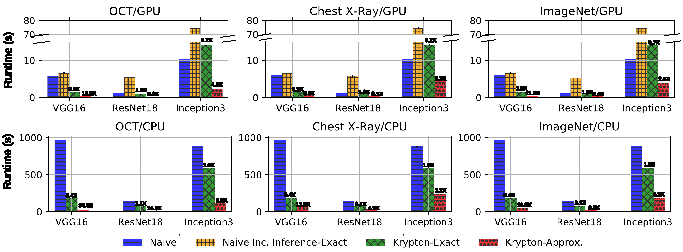
\includegraphics[width=\textwidth]{images/5_1_all_edited_b}
\vspace{-8mm}
\caption{End-to-end runtimes of \system~ and baselines on all 3 datasets, 3 CNNs, and both GPU and CPU.}
\label{fig:5_1_all_edited}
%\vspace{-2mm}
\end{figure*}

\vspace{2mm}
\noindent \textbf{Workloads.}
We use 3 diverse ImageNet-trained deep CNNs: VGG16~\cite{vggnet}, ResNet18~\cite{resnet}, and Inception3~\cite{inception}, obtained from~\cite{torchvisionmodels}. They complement each other in terms of model size, architectural complexity, computational cost, and our predicted theoretical speedups (Figure 3 in Section 3). For \textit{OCT} and \textit{Chest X-Ray}, the 3 CNNs were fine-tuned by retraining their final Fully-Connected layers as per standard practice. The details of fine-tuning are not relevant for the rest of our discussion; so, we present further details in the appendix. The OBE heatmaps are plotted using Python Matplotlib's \texttt{imshow} method using the \texttt{jet\_r} color scheme; we set the maximum threshold to \texttt{min}$(1, 1.25 p)$ and minimum to $0.75 p$, where $p$ is predicted class probability on a given image. All images are resized to the input size required by the CNNs ($224\times224$ for VGG16 and ResNet18; $299\times299$ for Inception3); no additional pre-processing was done. The GPU-based experiments used a batch size of $128$; for CPUs, the batch size was $16$. All CPU-based experiments were executed with a thread parallelism of $8$. All of our datasets, experimental scripts, and the \system~ codebase will be made publicly available on our project webpage.

\vspace{2mm}
\noindent \textbf{Experimental Setup.}
We use a machine with 32 GB RAM, Intel i7-6700 3.40GHz CPU, and NVIDIA Titan X (Pascal) GPU with 12 GB memory. %1 TB Seagate ST1000DM010-2EP1
The machine runs Ubuntu 16.04 with PyTorch version 0.4.0, CUDA version 9.0, and cuDNN version 7.1.2.
All reported runtimes are the average of 3 runs, with 95\% confidence intervals shown.

\vspace{-2mm}
\subsection{End-to- End Runtimes}\label{sec:end_to_end}

We focus on the most common OBE scenario of producing the whole heatmap; $G$ is automatically created (``non-interactive'' mode). We use an occlusion patch of size 16 and stride of 4. We compare two variants of \system: \system-Exact uses only incremental inference (Section 3), while \system-Approximate uses our approximate inference optimizations too (Section 4). The main baseline is \textit{Naive}, the current dominant practice of performing full inference for OBE with just only batching. We have another baseline on GPU: \textit{Naive Inc.~Inference-Exact}, which is a direct implementation of Algorithm~\ref{alg:incinference} in PyTorch/Python without using our GPU-optimized CUDA kernel (Section 3.4). Note that \textit{Naive Inc.~Inference-Exact} is not relevant on CPU.

We set the adaptive drill-down parameters based on the semantics of each dataset's prediction task (Section 4.3). For \textit{OCT}, since the region of interest is likely to be small, we set $r_{\mathit{drill}-\mathit{down}}=0.1$ and $\mathit{target} = 5$. For \textit{Chest X-Ray}, the region of interest can be large; so, we set $r_{\mathit{drill}-\mathit{down}} = 0.4$ and $\mathit{target} = 2$. For \textit{ImageNet}, which is in between, we use the \system~ default of $r_{\mathit{drill}-\mathit{down}}=0.25$  and $\mathit{target} = 3$. Throughout, $\tau$ is auto-tuned with a target SSIM of $0.9$ (Section 4.3). Figure~\ref{fig:5_1_all_edited} presents the results. Visual examples of the heatmaps produced are provided in the appendix.

Overall, we see \system~ offers significant speedups across the board on both GPU and CPU, with the highest speedups seen by \system-Approximate on \textit{OCT} with VGG16: $16$X on GPU and $34.5$X on CPU. The highest speedups of \system-Exact are also on VGG16: $3.9$X on GPU and $5.4$X on CPU. The speedups of \system-Exact are identical across datasets for a given CNN, since it does not depend on the image semantics, unlike \system-Approximate due to its parameters. \system-Approximate sees the highest speedups on \textit{OCT} because our auto-tuning yielded the lowest $r_{\mathit{drill}-\mathit{down}}$, highest target speedup, and lowest $\tau$ on that dataset. 

The speedups are lower with ResNet18 and Inception3 than VGG16 due to their architectural properties (kernel filter dimensions, stride, etc.) that make the projective field grow faster. Moreover, Inception3 has a complex DAG architecture with more branches and depth-wise concatenation, which limits GPU throughput for incremental inference. In fact, \system-Exact on GPU shows a minor slow-down ($0.7$X) with Inception3. But \system-Approximate still offers speedups on GPU with Inception3 (up to $4.5$X). We also see that ResNet18 and VGG16 almost near their theoretical speedups (Figure~\ref{fig:redundancy_ratio}) but Inception3 does not. Note that the theoretical speedup definition only counts FLOPs and does not account for memory stalls.

Finally, the speedups are higher on CPU than GPU; this is because CPU suffers less from memory stalls during incremental inferences. But the \textit{absolute} runtimes are much lower on GPU as expected. Overall, \system~ reduces OBE runtimes substantially for multiple datasets and deep CNNs. We also ran an experiment in the ``interactive'' mode by reducing $|G|$. As expected, speedups go down with $|G|$ due to the reduction in amortization benefits. Due to space constraints, these additional results are presented in the appendix.

\vspace{-2mm}
\subsection{Ablation Study}
We now analyze the contributions of our 3 optimizations individually. We compare the speedups of \system~ over \textit{Naive} (batched inference) on both CPU and GPU, termed  Empirical-CPU and Empirical-GPU respectively, against the theoretical speedups (explained in Sections 3 and 4).
% Does not matter. These experiments are dataset independent.
% All experiments use an image from the \textit{OCT} dataset (\red{TODO: Check}) and produce the full heatmaps.

\begin{figure}[t]
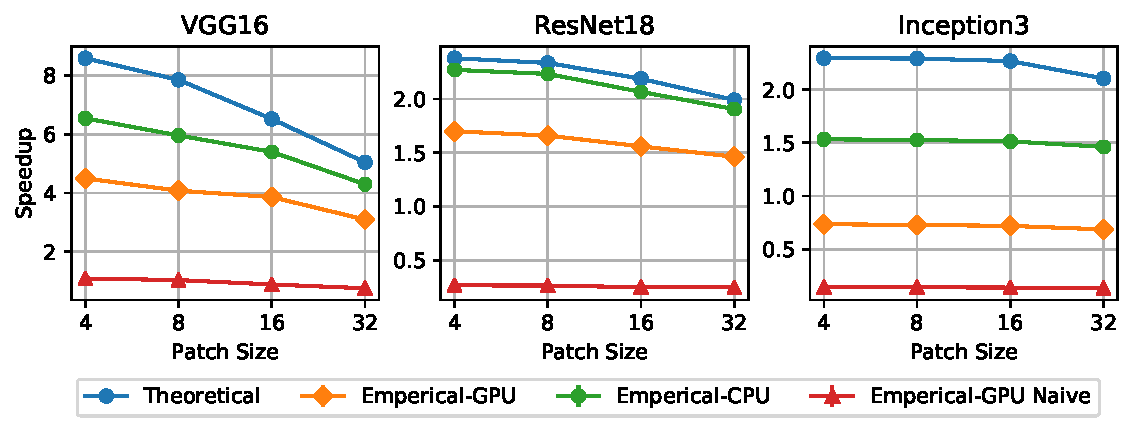
\includegraphics[width=\columnwidth]{images/5_2_1_edited}
\vspace{-8mm}
\caption{Speedups with only the incremental inference optimization (occlusion patch stride $S=4$).}
\vspace{-2mm}
\label{fig:5_2_1_edited}
\end{figure}

\vspace{2mm}
\noindent \textbf{Only Incremental Inference.} 
We vary the patch size and set the stride to $4$. Figure~\ref{fig:5_2_1_edited} shows the results. As expected, the speedups go down as the patch size increases. Empirical-GPU Naive yields no speedups because it does not use our GPU-optimized kernel, while Empirical-GPU does. But Empirical-CPU is closer to theoretical speedup and almost matches it on ResNet18. Thus, there is still some room for improvement to improve the efficiency of incremental inference in both environments.


\begin{figure}[t]
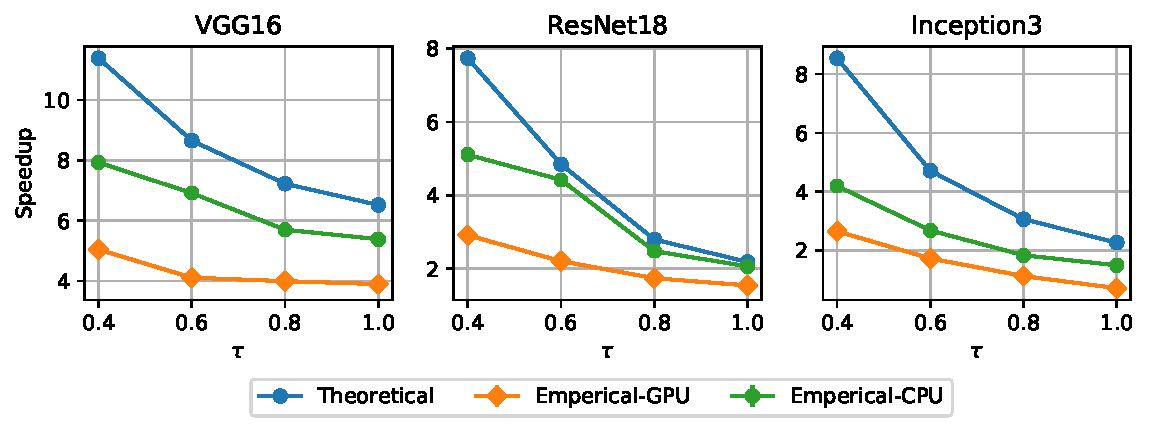
\includegraphics[width=\columnwidth]{images/5_2_2_edited}
\vspace{-8mm}
\caption{Speedups with incremental inference combined with only projective field thresholding.}
\vspace{-2mm}
\label{fig:5_2_2_edited}
\end{figure}

\vspace{2mm}
\noindent \textbf{Projective Field Thresholding.} We vary $\tau$ from $1.0$ (no approximation) to $0.4$. Adaptive drill-down is disabled but note that this optimization builds on top of our incremental inference. The occlusion patch size is $16$ and stride is $4$. Figure~\ref{fig:5_2_2_edited} shows the results. The speedups go up steadily as $\tau$ drops for all 3 CNNs. Once again, Empirical-CPU nears the theoretical speedups on ResNet18, but the gap between Empirical-GPU and Empirical-CPU remains due to the disproportionate impact of memory stalls on GPU. Overall, this approximation offers some speedups in both environments, but has a higher impact on CPU than GPU.

\begin{figure}[t]
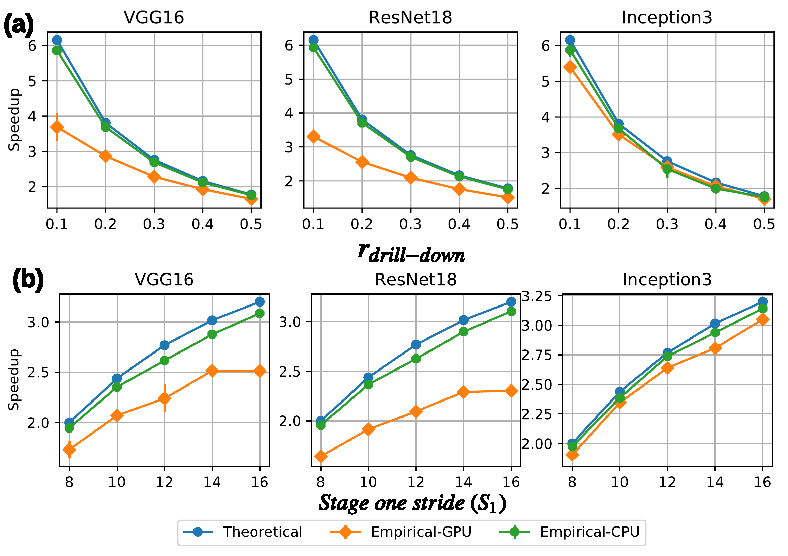
\includegraphics[width=\columnwidth]{images/5_2_3_edited}
\vspace{-8mm}
\caption{Speedups with incremental inference combined with adaptive drill-down. For (a), we set $S_1=16$. For (b), we set $r_{drill\_down}=0.25$).}
\vspace{-2mm}
\label{fig:5_2_3_edited}
\end{figure}

\vspace{2mm}
\noindent \textbf{Adaptive Drill-Down.} Finally we study the effects of adaptive drill-down (again, on top of incremental inference) and disable projective field thresholding. The occlusion patch size is $16$. Stage two stride is $S_2 = 4$. First, we vary $r_{drill-down}$, while fixing stage one stride ($S_1 = 16$). Figure~\ref{fig:5_2_3_edited} (a) shows the results. Next, we vary $S_1$, while fixing $r_{drill-down} = 0.25$. Figure~\ref{fig:5_2_3_edited} (b) shows the results. As expected, the speedups go up as $r_{drill-down}$ goes down or $S_1$ goes up, since fewer re-inference queries arise in both cases. Empirical-CPU almost matches the theoretical speedups across the board; in fact, even Empirical-GPU almost matches theoretical speedups on Inception3. Empirical-GPU flattens out at high $S_1$, since the number of re-inference queries drops, thus resulting in diminishing returns for the benefits of batched execution on GPU. Overall, this optimization has a major impact on speeding up OBE for all CNNs in both environments.


\vspace{2mm}
\noindent \textbf{Memory Overhead.} We compare our batched incremental inference against full re-inference on GPU. Our approach actually \textit{reduces} memory footprint by 58\%. Due to space constraints, we explain this result further in Appendix~\ref{sec:mem_overhead}.

% \vspace{-2mm}
% \subsection{\red{Other approaches for CNN prediction explanation and faster inference}}
% \red{
% We evaluate Axiomatic Attribution for Deep Networks method (a.k.a. integrated gradients method) \cite{sundararajan2017axiomatic} against OBE, which is also a popular approach for explaining CNN predictions.
% This method requires performing a series of forward-backward passes through the CNN to generate a sensitivity heatmap.
% The number of passes is determined by the \textit{steps} hyperparameter, which is usually set to value between 20 and 300.
% We evaluate integrated gradient method with 50 steps and OBE on three representative images from our datasets.
% The results are shown in Figure \ref{fig:igd}.
% }


\vspace{-2mm}
\subsection{Summary and Discussion}
Overall, our experiments show that \system~ can substantially accelerate OBE, with up to $16$X speedups on GPU and $34.5$X speedups on CPU. The benefits of our optimizations depend on the CNN's architectural properties. Our approximate inference optimizations also depend on the dataset's properties due to their tunable parameters, which \system ~can tune automatically. Finally, \system ~sees higher speedups on CPU than GPU but the runtimes are much lower on GPU. Overall, our optimizations in \system ~help reduce waiting times for OBE users by improving utilization of existing resources rather than forcing users to buy more resources.

While we focused on OBE in this paper to understand the benefits of IVM-based optimizations for CNNs, our ideas may be applicable to many other visual recognition tasks as well. For instance,~\cite{cavigelli2017cbinfer,buckler2018eva} exploit temporal locality in video, since successive frames do not differ much. One could integrate our ideas with theirs to devise new approximate IVM optimizations for CNNs. Going further, ``IVM-friendliness'' can be baked into the very model selection process that crafts the CNN architecture so that the model is both accurate and amenable to fast post-hoc explanations~\cite{motamedi2018resource}. However, such extensions require new techniques to batch update patches of arbitrary sizes and shapes, which requires deeper changes to \system. Thus, we leave them to future work.